\documentclass{article}

\usepackage{tikz}
\usepackage{xcolor}
\usepackage{multicol}
\usepackage{listings}
\usepackage[most]{tcolorbox}
\usepackage{parskip}
\usepackage{listings-rust}
\usepackage[scale=0.9]{sourcecodepro}
\usepackage{bytefield}
\usepackage{tikz}
\usetikzlibrary{arrows,calc,positioning}

\tikzstyle{intt}=[draw,text centered,minimum size=6em,text width=5.25cm,text height=0.34cm]
\tikzstyle{intl}=[draw,text centered,minimum size=2em,text width=2.75cm,text height=0.34cm]
\tikzstyle{int}=[draw,minimum size=2.5em,text centered,text width=3.5cm]
\tikzstyle{intg}=[draw,minimum size=3em,text centered,text width=6.cm]
\tikzstyle{sum}=[draw,shape=circle,inner sep=2pt,text centered,node distance=3.5cm]
\tikzstyle{summ}=[drawshape=circle,inner sep=4pt,text centered,node distance=3.cm]


% a4 marigns
\usepackage[a4paper, total={6in, 8in}]{geometry}


\tcbset {
  base/.style={
    arc=0mm,
    bottomtitle=0.5mm,
    boxsep=1mm,
    boxrule=0mm,
    colbacktitle=black!10!white,
    coltitle=black,
    fonttitle=\bfseries,
    left=2.5mm,
    leftrule=1mm,
    right=3.5mm,
    title={#1},
    toptitle=0.75mm,
  },
    sub/.style={
        base={#1},
        colframe=black!30!white,
        top=-0.5mm,
        bottom=-0.5mm,
    },
}

\definecolor{brandblue}{rgb}{0.34, 0.7, 1}
\newtcolorbox{mainbox}[1]{
  colframe=brandblue,
  base={#1}
}

\newtcolorbox{subbox}[1]{
  colframe=black!30!white,
  sub={#1}
}

% warning box
\newtcolorbox{warningbox}[1]{
  colframe=red,
  base={#1}
}

\usepackage{lato}
\renewcommand*\familydefault{\sfdefault}
\newcommand{\code}[1]{\texttt{#1}}
\usepackage[T1]{fontenc}
\usepackage{hyperref}
\usepackage{fancyhdr}

\pagestyle{fancy}
\fancyhf{}
\rhead{Giorgio Grigolo}
\lhead{Netsketch: A Collaborative Whiteboard}
\rfoot{Page \thepage}

\definecolor{bluekeywords}{rgb}{0.13, 0.13, 1}
\definecolor{greencomments}{rgb}{0, 0.5, 0}
\definecolor{redstrings}{rgb}{0.9, 0, 0}
\definecolor{graynumbers}{rgb}{0.5, 0.5, 0.5}


\lstset{
    commentstyle=\color{greencomments},
    keywordstyle=\color{bluekeywords},
    stringstyle=\color{redstrings},
    numberstyle=\color{graynumbers},
    % breaklines=true,
    basicstyle=\ttfamily,
    language=Rust,
    xleftmargin=.3\textwidth, xrightmargin=.3\textwidth,
    captionpos=b
}

\title{Netsketch: A Collaborative Whiteboard \\ { \Large Assignment Report} }
\author{Giorgio Grigolo}
\date{}

\hypersetup{
    colorlinks=true,
    linkcolor=blue,
    filecolor=magenta,
    urlcolor=blue,
}

\begin{document}

\maketitle
\tableofcontents

\newpage

\section{Introduction}
This implementation of Netsketch, a collaborative whiteboard, is built entirely in Rust, a statically typed, memory-safe, idiomatic, systems programming language.

\subsection{Project Structure}
Netsketch was divided into three main components: the \textit{server}, the \textit{client}, and a \textit{shared library}. The server is responsible for most of the business logic, such as managing the state of the whiteboard and broadcasting changes to all connected clients. The client is a graphical user interface that allows users to draw on the whiteboard and see the changes made by other users. The shared library contains the data structures and algorithms used by both the server and the client.

To conform with the Rust ecosystem's conventions, the above components are manifested as a Rust workspace, with the server and the client as separate crates, and the shared library as a library crate, initialized by the \code{cargo init {-}{-}lib} command.

\subsection{Libraries Used}
A considerable effort has been made to use as few external libraries (or
\textit{crates}) as possible. The only crates used are
\begin{itemize}
    \item \href{https://docs.rs/clap/latest/clap/}{\code{clap}} for the command-line interfaces of the server and the client,
    \item \href{https://docs.rs/thiserror/latest/thiserror/}{thiserror} for better error handling,
    \item \href{https://docs.rs/bincode/latest/bincode/}{\code{bincode}} for encoding and decoding data structures into and from bytes,
    \item \href{https://docs.rs/macroquad/latest/macroquad/}{\code{macroquad}} for the client's graphical user interface, and
    \item \href{https://docs.rs/tracing/latest/tracing/}{\code{tracing}} for pretty server side logging.
\end{itemize}
All other functionality has been implemented from scratch, or by using the Rust standard library \href{https://doc.rust-lang.org/std/}{\code{std}}.


% \newpage

\section{System Design}
It is clear, as specified, that this game is a client-server application. Upon
reading the requirements of this project, it was immediately clear that most of
the logic should take place on the server side, whereas the client, must be kept
as simple as possible; it must send clear and concise instructions to the server.
With this in mind, while planning the layout of this system, I concluded that
I'd like to keep the client as light as possible, while letting the server doing
most of the heavy lifting.

\subsection{Shared Library: \code{ns-core}}
In this section, I will describe the main features of the core of Netsketch, the library that is used by both the client and the server. I will also attempt to shed some light on the most important data structures in this library.

\subsubsection{Don't panic: \code{Error}}

One of the undesirable outcomes during the lifetime of a Rust program is the
\code{Panic}, more commonly known as crashing. To avoid this, I slightly
modified the common Rust concept of a \code{Result<T, E>}, where \code{T} is some Type, and \code{E} is some Error type.

In the shared library, with the help of \code{thiserror} crate, I renamed the default \code{Result} type, essentialy forcing the \code{Error} to be our own custom \code{ns\_core::Error}, and avoid filling it in everytime. The advantage of this is that we can define \textit{sub errors}, in an attempt to categorize them under the situation where they may be thrown. Most notably, we have at least an entry for each error returned by the crates we're using, as we want our \code{Result} type to understand as many errors we can, even if the \code{From} trait must be implemented manually. All this is to use the \code{?} notation instead of using too many \code{.unwrap()}s.


\label{sec:canvas}
\subsubsection{A blank slate: \code{Canvas}}

The central part of Netsketch is the interactive whiteboard, or \textit{canvas}, as I will
refer to it from now on. It is defined as an array of \textit{canvas entries},
and a monotonically increasing counter, to keep track of the order in which the
actions were performed, as well as to serve as a current pointer to the last
entry that was inserted into the canvas.

\begin{subbox}{}
    \begin{lstlisting}
struct Canvas {
    entries: Vec<CanvasEntry>,
    counter: usize,
}
        \end{lstlisting}
\end{subbox}

This calls the introduction of the \code{CanvasEntry}. The \code{CanvasEntry} stores the action's ID, the object drawn (the \code{CanvasElement}), the username of who drew it (the \code{author}), and a \code{shown} flag to be used by the client to determine whether the entry should be displayed or not.


\begin{subbox}{}
    \begin{lstlisting}
struct CanvasEntry {
    id: usize,
    element: CanvasElement,
    shown: bool,
    author: String,
}
\end{lstlisting}
\end{subbox}

The \code{CanvasElement}, finally is just an enum that contains all the possible objects that can be drawn on the canvas, and the required information to draw them such as sets of coordinates, colour and so on. The objects supported are \code{Line}, \code{Rectangle}, \code{Circle}, and \code{Text}.

\vspace{1em}

\begin{mainbox}{Note}
    The \code{Canvas} is further wrapped in another struct, which varies depending on the context in which it is used. In fact, the way it is mutated and accessed is different in the server and in the client. This will be discussed in the following sections.
\end{mainbox}

\newpage

\subsubsection{First signs of communication: \code{TcpPackets}}
Whilst planning how I'm going to transfer data between the client and the
server, I remembered I'm using Rust, which boasts an incredible type system. Indeed, enums in Rust are quite flexible, in the sense that one can define any arbitrary struct within the same enum entry. The \code{TcpPacket} system I implemented makes heavy use of this. At the network level, the packet structure is quite simple, as can be seen in figure \ref{fig:fig1}.

By splitting a packet in two main sections, we are able to exactly determine how
many bytes to read from the stream provided by a TCP socket, and therefore also
the size of the buffers which will be populated with the data.

In this way, we can make use of \code{read\_exact(\&mut [u8])}, a wrapper over the \code{read} system call, which keeps on reading from the stream until the mutable slice whose reference we pass to the function is full.

\begin{figure}[h]
    \centering
    \begin{bytefield}[bitwidth=3em]{4}
        \bitheader{0-3}\\
        \wordbox{1}{Payload Length} \\
        \wordbox{2}{Payload}
    \end{bytefield}
    \caption{TCP Packet Datagram}
    \label{fig:fig1}
\end{figure}

Over the wire, any element of the \code{TcpPacket} enum is sent as bits, or more conveniently as a \code{Vec<u8>}, byte-array. How do we decide the order in which to place the bytes of the data contained in each \code{TcpPacket} entry? Since we already noted that enums are quite flexible, in fact, completely arbitrary, it makes the contents quite unpredictable.

Fortunately, using some meta-programming (or Rust procedural macros) we are able
to uniquely encode structs into bits, given a translation table, or
mathematically speaking, a bijective function that recursively maps the types of
the members of the struct to the memory layout of the struct itself.

As per the \code{bincode}
\href{https://github.com/bincode-org/bincode/blob/trunk/docs/spec.md}{specification},
we note that by default, all structures are encoded in little-endian, with
various patterns for each data type. For example enums are encoded with their
variant first, followed by optionally the variant fields. The variant index is
based on the \code{IntEncoding} during serialization. For the
\code{IntEncoding}, by default, \code{bincode} uses a variable integer encoding
which means that the size of the integer is not fixed, but rather depends on the
value of the integer itself.

% \begin{enumerate}
%     \item If $u < 251$, encode it as a single byte with that value.
%     \item If $251 \leq u < 2^{16}$, encode it as a literal byte 251, followed by a u16 with value $u$.
%     \item If $2^{16} \leq u < 2^{32}$, encode it as a literal byte 252, followed by a u32 with value $u$.
%     \item If $2^{32} \leq u < 2^{64}$, encode it as a literal byte 253, followed by a u64 with value $u$.
%     \item If $2^{64} \leq u < 2^{128}$, encode it as a literal byte 254, followed by a u128 with value $u$.
% \end{enumerate}

% \texttt{usize} is being encoded/decoded as a \texttt{u64} and \texttt{isize} is being encoded/decoded as a \texttt{i64}.

All the rest is abstracted out in the \code{Encode} and \code{Decode} derive
macros respectively, which when applied to our \code{Packet} struct, they allow
us to use the \code{bincode::encode\_to\_vec} on the \code{Packet} on the
sender's side, and \code{bincode::decode\_from\_slice} on the receiving end,
whilst casting the decode function call to the \code{Packet} enum. This is
because \code{bincode} is just receiving bytes: it is not aware how they are to
be arranged, until we give it a type hint. Due to the fact that we are allowed to cast
any bytes to any struct, this process might fail, which is why the
\code{try\_from\_bytes} function implemented for a \code{Packet} returns a \code{Result}.

{
\lstset{xleftmargin=0\textwidth, xrightmargin=0\textwidth}
\begin{subbox}{}
    \begin{lstlisting}[language=Rust]
impl Packet { ...
fn try_from_bytes(bytes: &[u8]) -> Result<Self> {
    Ok(bincode::decode_from_slice(bytes, config::standard())?.0)
}
... }
\end{lstlisting}
\end{subbox}
}

\newpage

\subsection{The Server: \code{ns-server}}

During the initial brainstorming sessions, it was clear to me that whenever a
client drew on the canvas, sending the entire data structure to everyone over
and over again was going to be quite inefficient. In this section, I will
outline the main execution flow of the server, how it handles incoming packets,
and most importantly, how it concurrently manages its state safely, amongst all
clients.

Thankfully, it was an early stage where I made the foundational design decision
whereby only the updates to the canvas had to be propagated to the clients'
canvases. It was also apparent that I had to implement a cached version of the
canvas for the client, as well as an \textit{update receiver} to keep the canvas
up to date. We shall talk about the client-specific implementations in a
subsequent section.


\subsubsection{Sharing is caring: \code{Arc<Mutex<T>{>}}}

When handling incoming connections, the sever spawns a new thread for each
connection. This is done to avoid blocking the main thread, and to allow the
server to handle multiple clients concurrently. However, at least in Rust, it is
not possible to share mutable data between threads without some form of
synchronization and a method to allow us to share value ownership.  The
\code{Arc<Mutex<T>>} pattern is a common way to achieve this.

The \code{Arc} is an \textit{atomically reference-counted pointer}, which allows
us to safely share the ownership of a value across multiple threads.When cloning
an \code{Arc} an new instance that points to the same heap allocation as the
original Arc is created, whilst incrementing the reference count. Finally, when the last
Arc pointer to a specific allocation is disposed of, the value in that
allocation is also dropped.

\begin{mainbox}{Note}
    \code{Arc} does not ensure thread safety by itself, it only protects against
    race conditions when sharing ownership. An example of this is when a thread
    tries to clone an \code{Arc} while another thread is dropping it.
\end{mainbox}

However, in Rust, shared references prohibit mutation by default, and since
\code{Arc} is a shared reference, we need to further wrap our inner data
structure in a \code{Mutex} to allow for mutation, particularly amongst multiple
threads. The \code{Mutex} is a mutual exclusion primitive provided by the Rust
standard library, which allows us to lock and unlock the canvas, ensuring that
only one thread can access and modify it at a time.

In essence, we are putting clients into a metaphorical queue, where they are
allowed to access the canvas one by one, and only when they are done, the next
client in the queue is allowed to access the canvas. This, inevitably introduces
some latency, as well as an inferred order in which the operations on the canvas
are performed.

\begin{subbox}{}
    \lstset{xleftmargin=0\textwidth, xrightmargin=0\textwidth}
    \begin{lstlisting}[language=Rust]
let mut server_state = match server_state.lock() {
        Ok(server_state) => server_state,
        Err(_) => return Err(ServerError::LockError.into()),
};
    \end{lstlisting}
\end{subbox}

The code snippet above demonstrates the \code{handle\_client} function. It spawns a
thread for client-requested operations, secures the canvas, or errors if the
lock fails.  This ensures thread safety and mutual exclusivity, for the server's
the critical section - canvas mutation. Conveniently, Rust unlocks the mutex
automatically when the scope of the lock ends.

\label{sec:serverstate}
\subsubsection{What we are sharing: \code{ServerState}}

Now that we know how the server state is passed \textit{safely} to a thread, we
can observe what it is storing, and most importantly why. In this section, we
will discuss the \code{ServerState} struct, which is the main data structure
that the server uses to manage the state of the whiteboard, as well as the
clients connected to it.

\begin{subbox}{}
    \lstset{xleftmargin=0.2\textwidth, xrightmargin=0.2\textwidth}
    \begin{lstlisting}[language=Rust]
struct ServerState {
    canvas: Canvas,
    sessions: Vec<Session>,
    users: HashMap<String, UserData>,
}
    \end{lstlisting}
\end{subbox}

The \code{ServerState} struct contains the canvas (see Section
\ref{sec:canvas}), a list of sessions, and a map of usernames to the
respective user data.

\begin{subbox}{}
    \lstset{xleftmargin=0.2\textwidth, xrightmargin=0.2\textwidth}
    \begin{lstlisting}[language=Rust]
 struct Session {
     username: String,
     stream: TcpStream,
}
    \end{lstlisting}
\end{subbox}

The \code{Session} struct contains two fields: the \code{username} of the client
and the \code{TCPStream} that the client is connected to. The
\code{std::net::TCPStream}s found in this list of sessions are what the server
uses to broadcast canvas updates to the clients.

\begin{subbox}{}
    \lstset{xleftmargin=0.2\textwidth, xrightmargin=0.2\textwidth}
    \begin{lstlisting}[language=Rust]
struct UserData {
        username: String,
        action_history: Vec<Action>,
        last_login: Option<Instant>,
    }
\end{lstlisting}
\end{subbox}

The \code{UserData} struct contains the client's username, their \code{Action}
history (for the \textit{undo} logic) and the last login time, which is used to
determine when the server should adopt the client's action history. I have
augmented the \textit{draw list} as found in the assignment specification to an
action history, which includes not just a series of \code{Draw} commands, but
also \code{Delete}, \code{Clear} and \code{Update} commands.

\newpage

\subsubsection{The main \textit{(for)} loop}

With all the data structures in place, we can now discuss the main execution
flow of the server.

Firstly, we call \code{init\_server}, which does the following:
\begin{itemize}
    \item Starts a subscriber for tracing events, which is used for logging.
    \item Binds the server to the specified address.
    \item Returns the TCP listener, which is used to accept incoming connections.
\end{itemize}

Secondly, we initialize the server state, as previously described (see Section \ref{sec:serverstate}).

Finally, we enter the main \textit{for} loop, where we iterate over
\code{tcp\_listener.incoming()}, which as the Rust documentation states, is
equivalent to calling \code{TcpListener::accept} in a loop. This \code{accept}
method, is the same as the \code{accept} system call found in
\code{sys/socket.h} in C, which blocks until a new connection is made to the
server.

For this reason, we spawn a new thread for each incoming connection, inside
which we loop indefinitely whilst running the \code{handle\_client} function,
which is responsible for handling the client's requests. If for any reason, the
\code{handle\_client} function returns an error, the server will log the error
disconnect the user (by removing the session) and continue to the next iteration
of the loop.

\begin{warningbox}{Limitation}
    It is possible, that the server could be overwhelmed by the number of clients
    connected to it, as it spawns a new thread for each connection. This could
    lead to a situation where the server runs out of resources, and the system
    becomes unresponsive. To mitigate this, the server could be modified to use a
    thread pool, which would limit the number of threads that can be spawned at
    any given time.
\end{warningbox}

To completely unravel the server's execution flow, all that is left is to
implement the \code{handle\_client} function. Firstly, we set up the client's
\code{TcpStream} to timeout after 10 minutes, which is the maximum time a client
can be inactive before being disconnected. We then read the first 4 bytes from
the stream, which contain the length of the payload, and then read the payload
itself. The thread will block until the payload is received, or until the
timeout is reached.

Once the payload is received, we decode it into a \code{Packet} enum, which
contains the client's request. Then we immediately lock the mutex containing the
server state, as we're entering the critical section. Next is arguably the most
important part of the server. Firstly, we check whether the user has an existing
session. If there is one, any type of packet is accepted, otherwise only a
connect packet is expected, to create the session. Secondly, we perform pattern
matching on the \code{Packet} enum and modify the canvas accordingly. One can
think of a Rust \code{match} statement as a glorified switch case. After the
canvas logic is performed, we \textit{broadcast} the update to every connected
client that is being kept track of in the session. These broadcasted packets are
identified by a subset of the \code{TcpPacket} enum, namely the \code{Response}
packets.

If the user sends a packet, but he does not have an entry in the \code{UserData}
hashmap, we expect different behaviour. In that case, we only expect a
\code{Connect} packet, which is the only packet that is allowed to be sent by a
client that is not connected to the server. Otherwise, the server will log an
error and disconnect the client.

\newpage

\subsection{The Client: \code{ns-client}}

In this section we will discuss the client's implementation, and how it
interacts with the server. The client is a mixture of a command-line and
graphical interface, where the user issues commands to the server via the
command-line interface, and displays the canvas on a window generated by the
graphics library \code{macroquad}.


This time, we use a combination of message passing, multithreading and the
\textit{multiple-sender-single-consumer} design pattern.

As illustrated in Figure \ref{fig:interaction_diagram}, the client spawns three
threads, each responsible for a different task. The main thread is responsible
for receiving input handling the command-line interface, the TCP
handler thread is responsible for sending and receiving packets to and from the
server, and the canvas thread is responsible for rendering the canvas on the
screen.

\begin{figure}[!htb]
    \centering
    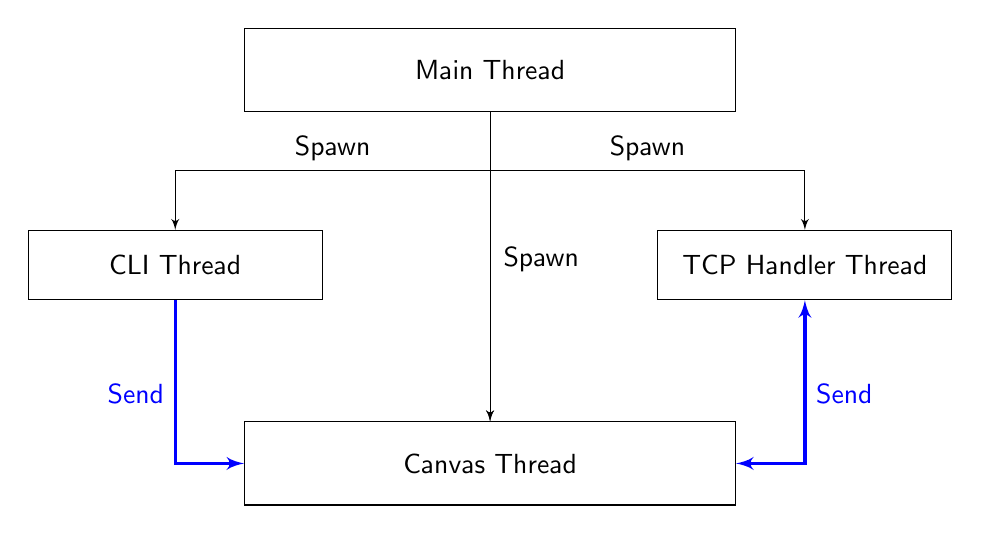
\begin{tikzpicture}[
            >=latex',
            auto
        ]
        \node [intg] (kp)  {Main Thread};
        \node [int]  (ki1) [node distance=1.5cm and -1cm,below right=of kp] {TCP Handler Thread};
        \node [int]  (ki2) [node distance=1.5cm and -1cm,below left=of kp] {CLI Thread};
        \node [intg] (ki3) [node distance=5cm,below of=kp] {Canvas Thread};
        \draw[->] (kp) -- ($(kp.south)+(0,-0.75)$) -| (ki1) node[above,pos=0.25] {Spawn} ;
        \draw[->] (kp) -- ($(kp.south)+(0,-0.75)$) -| (ki2) node[above,pos=0.25] {Spawn} ;
        \draw[->] (kp) -- (ki3) node[above,pos=0.55, xshift=0.65cm] {Spawn} ;
        \draw[blue, very thick, <->] (ki1) |- (ki3) node[above,pos=0.35, xshift=0.5cm] {Send} ;
        \draw[blue, very thick, ->] (ki2) |- (ki3) node[above,pos=0.35, xshift=-0.5cm] {Send} ;
        \draw[->] (kp) -- (ki3);
    \end{tikzpicture}
    \caption{Client Interaction Diagram}
    \label{fig:interaction_diagram}
\end{figure}

\subsubsection{TCP Handler Thread}

In this thread the client creates an instance of a \code{TcpStream}, and spawns
two threads to handle reading and writing to the stream. The main reason for
this is so that when the client draws something on the canvas, it can send the
packet to the server, whilst receiving updates from the server at the same time.

How does the client know when to send a packet to the server, if the thing that
handles all the packets is isolated in a different thread? The answer is by using a
\textit{multiple-sender-single-consumer} (MPSC) channel. Before creating the thread, we
initialize an MPSC channel, creating a (cloneable) sender, and a receiver. The
receiver is passed to the TCP handler thread, and the sender is passed to all
the other threads that need to send packets to the server.

This design patterns allows us to send packets to the server from any thread,
whilst seperating concerns and keeping the code clean and modular.

\subsubsection{Canvas Thread}





\end{document}
